\begin{center}
    
\begin{tikzpicture}[x=6em, y=1.5em,baseline=0.5em]
    \draw[very thick] (0,0)--(1,0) (1,3)--(0,3)--(0,0);
    \end{tikzpicture} \hspace{2em}
    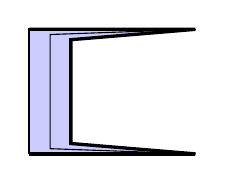
\begin{tikzpicture}[x=6em, y=1.5em,baseline=0.5em]
    \draw[very thick] (0,0)--(1,0) (1,3)--(0,3)--(0,0);
    \def\n{8}
    \def\t{2}
    \def\m{1/\n}
    \foreach \i in {\t,...,0}{
        % the first point is (x, x)
        % the second one is (x, 3-x)
        \filldraw[fill=blue!20] (0,0)--(1,0)--(\i*\m,\i*\m)--(\i*\m, 3-\i*\m)--(1,3)--(0,3);
    }
    \draw[very thick] (0,0)--(1,0)--(\t*\m,\t*\m)--(\t*\m, 3-\t*\m)--(1,3)--(0,3);
    \end{tikzpicture} \hspace{2em}
    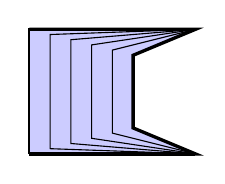
\begin{tikzpicture}[x=6em, y=1.5em,baseline=0.5em]
    \draw[very thick] (0,0)--(1,0) (1,3)--(0,3)--(0,0);
    \def\n{8}
    \def\t{5}
    \def\m{1/\n}
    \foreach \i in {\t,...,0}{
        % the first point is (x, x)
        % the second one is (x, 3-x)
        \filldraw[fill=blue!20] (0,0)--(1,0)--(\i*\m,\i*\m)--(\i*\m, 3-\i*\m)--(1,3)--(0,3);
    }
    \draw[very thick] (0,0)--(1,0)--(\t*\m,\t*\m)--(\t*\m, 3-\t*\m)--(1,3)--(0,3);
    \end{tikzpicture} \hspace{2em}
    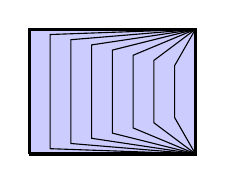
\begin{tikzpicture}[x=6em, y=1.5em,baseline=0.5em]
    \filldraw[very thick, fill=blue!20] (0,0)--(1,0)--(1,3)--(0,3)--(0,0);
    \def\n{8}
    \foreach \i in {0,...,\n}{
        \def\m{1/\n}
        % the first point is (x, x)
        % the second one is (x, 3-x)
        \draw (1,0)--(\i*\m,\i*\m)--(\i*\m, 3-\i*\m)--(1,3);
    }
    \end{tikzpicture}
\end{center}